% A group as a one-object category: every arrow is an isomorphism.
% Source: book/tex/cats/categories.tex (§ Definition and examples).
\documentclass[border=2mm]{standalone}
\usepackage{tikz}
\usetikzlibrary{arrows.meta}
\newcommand{\id}{\mathrm{id}}
\begin{document}
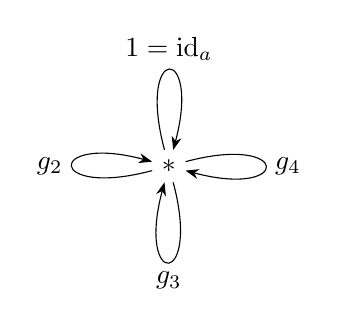
\begin{tikzpicture}[>=Stealth, every loop/.style={min distance=14mm, looseness=18}]
  \node (a) at (0,0) {$\ast$};
  \draw[->] (a) to[loop above] node[above]{$1=\id_a$} (a);
  \draw[->] (a) to[loop left]  node[left]{$g_2$} (a);
  \draw[->] (a) to[loop below] node[below]{$g_3$} (a);
  \draw[->] (a) to[loop right] node[right]{$g_4$} (a);
\end{tikzpicture}
\end{document}
